\providecommand{\main}{..}
\documentclass[\main/notes.tex]{subfiles}

\begin{document}
	\setcounter{chapter}{9}
	\chapter{Software Engineering}
		\section{Software Lifecycle}
			\begin{definition}{Software Lifecycle}
				\begin{enumerate}
					\item Software is developed by a group of developers
					\item Software is used for a while.
					\item Software modifications become necessary, either due to errors, changes in laws, or changes in the company.
					\item Software is used and modified.
					\item Software becomes obsolete
						\begin{indentparagraph}
							\begin{description}
								\item[Obsolete] The software loses its validity due to inefficiency, obsolence of the language, major changes in user requirements, or other factors.
							\end{description}
						\end{indentparagraph}
				\end{enumerate}
				\begin{center}
					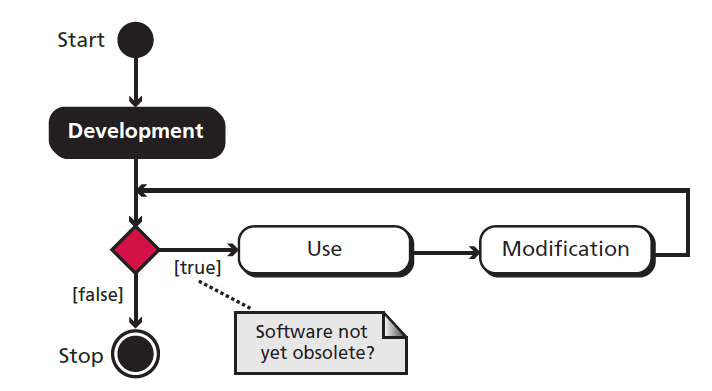
\includegraphics[width=0.8\textwidth]{\main/images/unit10/software_lifecycle.png}
				\end{center}
			\end{definition}
			\subsection{Development Process Models}
				The \concept{development process} involves four phases: \concept{analysis}, \concept{design}, \concept{implementation}, \concept{testing}. There are many models that contain these phases, the two most common are the \concept{waterfall model} and the \concept{incremental model}.
				\subsubsection{Waterfall Model}
					The development process flows in only one direction. A phase \emph{cannot} be started until a previous phase is complete.
					\begin{center}
						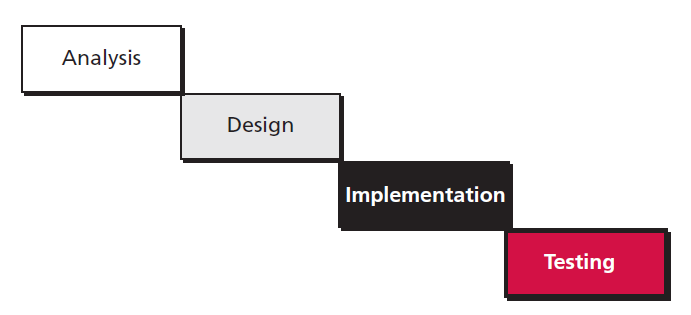
\includegraphics[width=0.6\textwidth]{\main/images/unit10/waterfall_model.png}
					\end{center}
					\begin{indentparagraph}
						\begin{description}
							\item[Advantages] Each phase is completed before the next phase starts. The testing phase can test the entire system.
							\item[Disadvantages] Difficulty in locating a problem -- harder to determine in which phase the problem appeared, so the entire process must be checked.
						\end{description}
					\end{indentparagraph}
				\subsubsection{Incremental Model}
					Softwaee is developed in a series of steps. The developers first complete a simplified version of the whole system, but without the details. On each iteration, more details are added.
					\begin{center}
						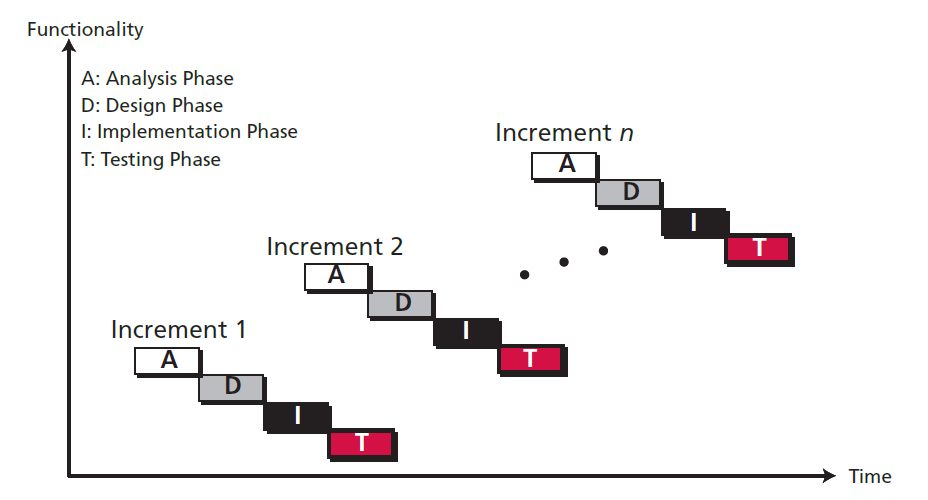
\includegraphics[width=0.8\textwidth]{\main/images/unit10/incremental_model.png}
					\end{center}
					\begin{indentparagraph}
						\begin{description}
							\item[Advantages] If a problem occurs, the developers know that it is to do with new functionality.
							\item[Disadvantages] Can be a neverending process, as new functionality can always be added.
						\end{description}
					\end{indentparagraph}

		\section{Analysis Phase}
			\begin{definition}{Analysis Phase}
				Results in a specification document that shows \emph{what} the software will do, without specifying \emph{how} it will be done. The approaches used depend on whether the implementation phase will be come using a procedural programming language, or an object-oriented language.
			\end{definition}
			\subsection{Procedure-Oriented Analysis}
				Also called \concept{structural analysis} or \concept{classical analysis}. Used if the implementation phase will use a procedural language.
				\begin{definition}{Data Flow Diagrams}
					Show the movement of data in the system. Use four symbols: a square box is the source or destination, a rectangle with rounded corners is the process, an open-ended rectangle shows where the data is stored, and arrows show the flow of data.
					\begin{center}
						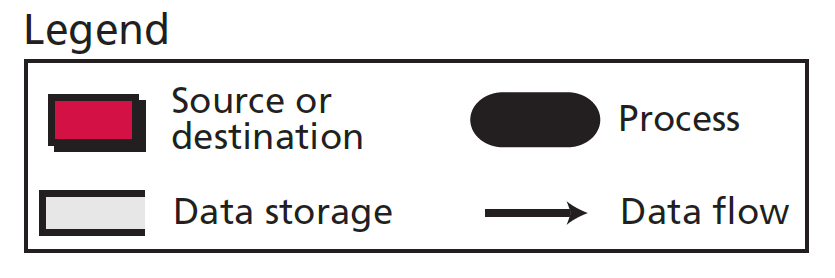
\includegraphics[width=0.5\textwidth]{\main/images/unit10/data_flow_symbols.png}
					\end{center}
				\end{definition}
				\begin{definition}{Entity-Relationship Diagrams}
					Also used in database design. Shows the entities for which information needs to be stored, and the relationship between those entities.

					Rectanges represent entity sets. Ellipses represent attributes. Diamonds represent relationship sets. Lines link attributes to entity sets, and link entity sets to relation sets.

					\begin{center}
						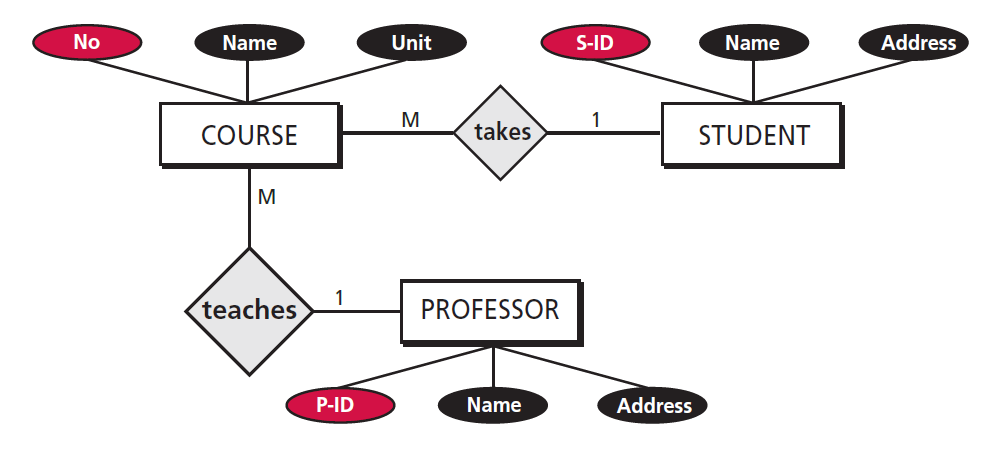
\includegraphics[width=0.7\textwidth]{\main/images/unit10/entity_relationship_example.png}
					\end{center}
				\end{definition}
				\pagebreak
				\begin{definition}{State Diagrams}
					Used when the state of an entity in the system will change in response to events.

					Example for an elevator:
					\begin{center}
						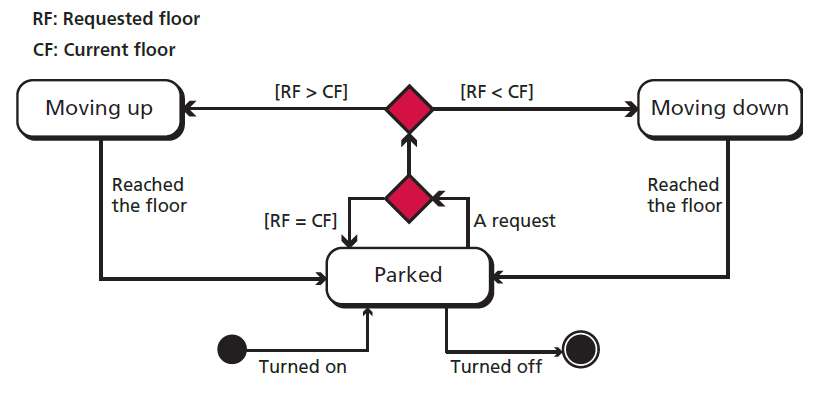
\includegraphics[width=0.7\textwidth]{\main/images/unit10/state_diagram_elevator.png}
					\end{center}
				\end{definition}
			\subsection{Object-Oriented Analysis}
				Used if the implementation phase will use an OO language.
				\begin{definition}{Use-case Diagrams}
					Gives the user's view of a system: shows how the user communicates with the system. Uses four components: \concept{system}, \concept{use cases}, \concept{actors}, and \concept{relationships}.
					\begin{indentparagraph}
						\begin{description}[nosep]
							\item[System] Shown with a rectangle. Performs a function.
							\item[Use cases] Shown with rounded rectangles. Actions in the system.
							\item[Actor] Shown with a stick figure. Someone or something that uses the system. Not necessarily a human.
						\end{description}
					\end{indentparagraph}
					\begin{center}
						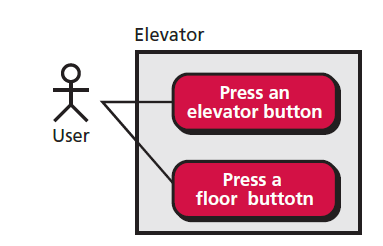
\includegraphics[width=0.4\textwidth]{\main/images/unit10/use_case_diagram_elevator.png}
					\end{center}
				\end{definition}
				\pagebreak
				\begin{definition}{Class Diagrams}
					Determine the entities involved in the system, and how the entities are related to each other. Use the concepts of \concept{is-a} for inheritance, and \concept{has-a} for how different objects are related.
					\begin{center}
						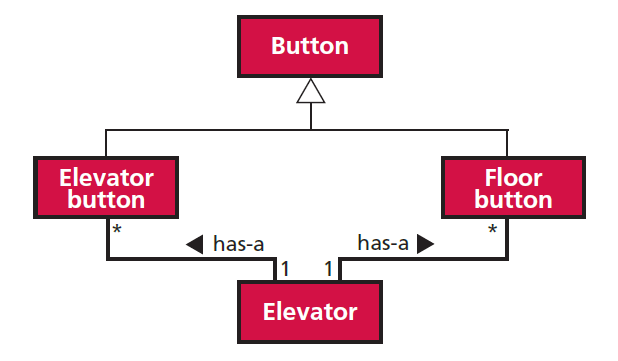
\includegraphics[width=0.6\textwidth]{\main/images/unit10/class_diagram_elevator.png}
					\end{center}
				\end{definition}
				\begin{definition}{State Chart}
					Plays the same role as the state diagram in procedure-oriented analysis.
				\end{definition}

		\section{Design Phase}
			\begin{definition}{Design Phase}
				Defines \emph{how} the system will accomplish what was defined in the analysis phase. All components of the system are defined.
			\end{definition}
			\subsection{Procedure-Oriented Design}
				Design both procedures and data. The whole system is divided into a set of procedures or modules.
				\begin{definition}{Structure Chart}
					Illustrates the relationships between modules. An example for an elevator:
					\begin{center}
						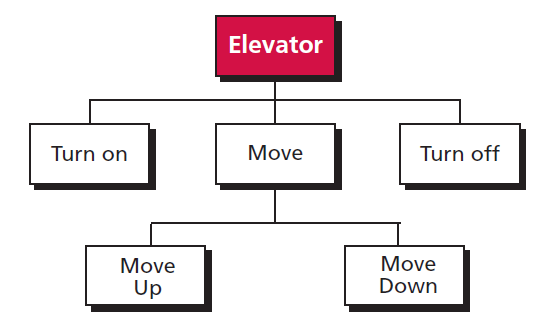
\includegraphics[width=0.5\textwidth]{\main/images/unit10/structure_chart_elevator.png}
					\end{center}
				\end{definition}
				\subsubsection{Modularity}
					\begin{definition}{Modularity}
						Breaking a large project into smaller parts that can be understood and handles easily. Two main concerns when a system is divided into modules: \concept{coupling} and \concept{cohesion}.
					\end{definition}
					\begin{definition}{Coupling}
						A measure of how tightly two modules are bound to each other. Must be \emph{minimised}, as
						\begin{itemize}[nosep]
							\item loosely coupled modules are more reusable
							\item loosely coupled modules are less likely to create errors in related modules
							\item when modifications are needed, only the modules that need to change are affected
						\end{itemize}
					\end{definition}
					\begin{definition}{Cohesion}
						A measure of how closely the modules in a system are related. Must be \emph{maximised}.
					\end{definition}
			\subsection{Object-Oriented Design}
				Elaborate the details of classes. Classes are made of a set of variables (\concept{attributes}) and a set of functions (\concept{methods}).

				List the details of the attributes and methods. For example:
				\begin{center}
					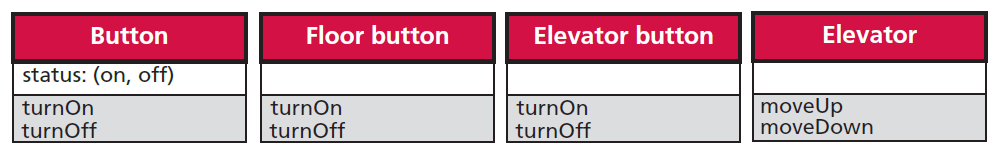
\includegraphics[width=0.8\textwidth]{\main/images/unit10/class_details_elevator.png}
				\end{center}

		\pagebreak
		\section{Implementation Phase}
			Programmers write the code for the modules in procedural programming, or write the units to implement classes in OO design. There are various issues to consider:
			\subsection{Language Choice}
				For procedural programming, normally a purely procedural language is chosen. For OO, both C++ and Java are common.
			\subsection{Software Quality}
				High quality software is software that meets the user's requirements, meets the operating standards for the organisation, and runs efficiently on the hardware for which it was developed. There are three main factora: \concept{operability}, \concept{maintainability}, and \concept{transferability}.
				\begin{center}
					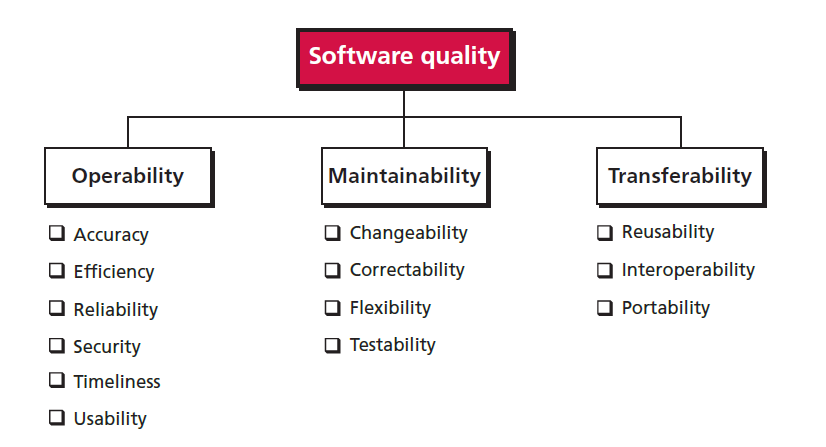
\includegraphics[width=\textwidth]{\main/images/unit10/software_quality_factors.png}
				\end{center}
				\pagebreak
				\subsubsection{Operability}
					\begin{definition}{Operability}
						The basic operation of a system.
					\end{definition}
					\begin{description}
						\item[Accuracy] Information is correct and error-free. Measured using metrics such as mean time between failures, number of bugs per thousand lines of code, and number of user requests for change.
						\item[Effeciency] Subjective term for the speed of the program. A user might specify a performance standard, which is then measurable.
						\item[Reliability] The sum of the other factors -- if users can count on the system, it is most likely reliable.
						\item[Security] How easy it is for unauthoried people to access the system's data. There are checklists to test this.
						\item[Timeliness] Is the response time reasonable? Is the output delivered timeously?
						\item[Usability] How easy it is for a user to use the system. Subjective.
					\end{description}
				\subsubsection{Maintainability}
					\begin{definition}{Maintainability}
						The ease with which a system can be kept up to data and running correctly.
					\end{definition}
					\begin{description}
						\item[Changeability] Subjective. The ease with which a requested change can be implemented. There are software measurement tools that will estimate a program's complexity and structure.
						\item[Correctability] The ease with which a program can be corrected if it fails.
						\item[Flexibility] Qualitative attribute measuring how easy it is to make changes.
						\item[Testability] How easy it is to test the program.
					\end{description}
				\subsubsection{Transferability}
					\begin{definition}{Transferability}
							The ability to move data and/or a system from one platform to another, and to reuse code.
					\end{definition}
					\begin{description}
						\item[Reusability] Modules are written so that they can be reused in other systems. For example, building a library of functions that can be used in different programs.
						\item[Interoperability] Ability to send data to other software systems.
						\item[Portability] Ability to move software from one hardware platform to another.
					\end{description}

		\pagebreak
		\section{Testing Phase}
			Find errors in the system. There are two types: \concept{glass-box} and \concept{black-box}.
			\begin{center}
				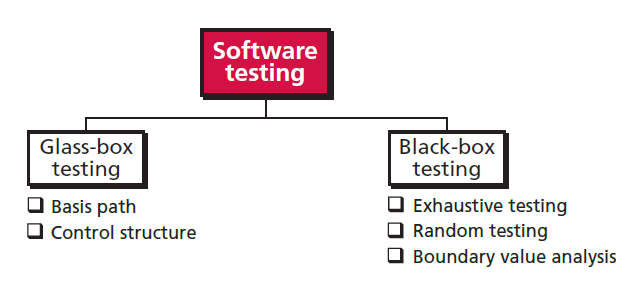
\includegraphics[width=0.7\textwidth]{\main/images/unit10/software_testing.png}
			\end{center}
			\subsection{Glass-Box Testing}
				Also called \concept{white-box testing}. Based on knowing the internal structure of the software. The goal is to determine whether all the components of the software do what they are designed to do.

				Assumes the tester knows everything about the software -- done by the software engineer or a dedicated team.

				Uses the structure of the software to guarantee that:
				\begin{itemize}[nosep]
					\item All independent paths in every module are tested at least once.
					\item All the decision constructs are tested on each branch.
					\item Each loop construct is tested.
					\item All data structures are tested.
				\end{itemize}
				\subsubsection{Basis Path Testing}
					\begin{definition}{Basis Path Testing}
							Proposed by Tom McCabe. Creates a set of test cases that executes \emph{every statement} in the software at least once.

							Uses \concept{graph theory} and \concept{cyclomatic complexity} to find the independent paths.
					\end{definition}
				\subsubsection{Control Structure Testing}
					More comprehensive than Basis Path Testing, and includes it. Uses different test categories:
					\begin{indentparagraph}
						\begin{description}
							\item[Condition Testing] Applies to any condition in the module. Designed to check whether all conditions are set correctly. A \concept{simple condition} is a relational expression, while a \concept{compund condition} is a combination of simple conditions and logical operators.
							\item[Data Flow Testing] Based on the flow of data through the module. Selects test cases that involve checking the value of variables when they are used on the left side of an assignment statement.
							\item[Loop Testing] Use test cases to check the validity of loops.
						\end{description}
					\end{indentparagraph}
			\subsection{Black-Box Testing}
				Testing software without knowing the internal structure. Tests the functionality of the software in terms of what the software is supposed to accomplish, such as its inputs and outputs.
				\begin{definition}{Exhaustive Testing}
					Test the software for all possible input values. This is normally too big, and therefore impractical.
				\end{definition}
				\begin{definition}{Random Testing}
						Use a subset of possible input values to test the output is correct. Important to ensure the values are distributed over the input domain properly.
				\end{definition}
				\begin{definition}{Boundary-value Testing}
					Test the values that are at the boundaries -- if a module requires a specific range, test the top and bottom of the range.
				\end{definition}

		\section{Documentation}
			Used to ensure software is used properly, and manintained effectively. This is an ongiong process. Only stops when the package becomes obsolete.
			\subsection{User Documentation}
				Shows users how to use the software -- often have a tutorial section that walks through each feature. Traditionally called a \concept{user guide}. Can be a powerful marketing tool.

				Should be written for both novice and expert users.
			\subsection{System Documentation}
				Defines the software itself. Should be written so that other developers can maintain and modify the software. Should exist for all four phases of development.
				\begin{indentparagraph}
					\begin{description}[nosep]
						\item[Analysis Phase] Information collected should be carefull documented, and should define the sources of the information.
						\item[Design Phase] The tools used in the final copy must be documented.
						\item[Implementation Phase] Every module of the code should be documented. The code should be self-documenting as far as possible, using comments, descriptive headers, and variable names.
						\item[Testing Phase] Each type of test applied should be mentioned, along with its result. This includes unfavourable results, and the data that produced them.
					\end{description}
				\end{indentparagraph}
			\subsection{Technical Documentation}
				Describe the installation and the servicing of the software.

		\rulechapterend
\end{document}